\section{Scene Format}

\begin{figure*}[htb]
\begin{center}
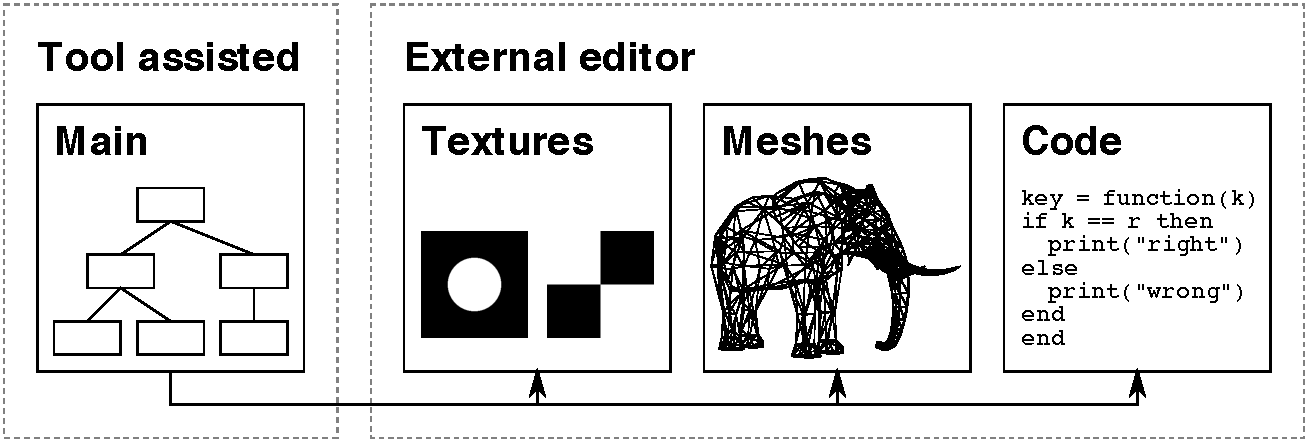
\includegraphics[width=15.5cm]{media/document.pdf}
\caption{Test scenes can consist of several files that contain the scene description and file pointers, textures, meshes or code.\label{imgDocument}}
\end{center}
\end{figure*}

\paragraph{}
The file format of test scenes has evolved a lot during development.
For a long time it was a free form LUA program, that had no constraints besides being valid LUA.
The programmer of the test had the responsibility to build up the scene graph, set the correct textures, load meshes, and register the desired event handlers.

\paragraph{Managed Main File}
This kind of scene file is still supported, but when creating a test with the UI tool, a different style has to be used.

The scene graph containing all objects including texture and camera settings is generated by \ER, so no custom code can be stored in the main file.
Textures and mesh files are referenced by the main file.
Those media files get loaded when building the scene graph.

Code also has to be referenced by the main file and stored in additional files.
When a scene is exported from the tool, the complete file is regenerated, changes made by the user are not honored outside their influence on the scene graph.
External file references however are tracked and exported along with the scene graph creation.
The user interface offers easy controls to add additional code files, all custom code should reside in them.

